% Unofficial University of Texas at Arlington Math Poster template:

% A fork of the unofficial University of Lethbridge Poster template: https://www.overleaf.com/latex/templates/university-of-lethbridge-unofficial-poster-template/nddfzgvqvfwf
% which is a fork of unofficial University of Alberta Poster template: 
% which is a fork of Yale template: https://www.overleaf.com/latex/templates/yale-poster-template/rjpgqfgvsjcv
% which is a fork of the UMich template https://www.overleaf.com/latex/templates/university-of-michigan-umich-poster-template/xpnqzzxwbjzc
% which is fork of the MSU template https://www.overleaf.com/latex/templates/an-unofficial-poster-template-for-michigan-state-university/wnymbgpxnnwd
% which is a fork of https://www.overleaf.com/latex/templates/an-unofficial-poster-template-for-new-york-university/krgqtqmzdqhg
% which is a fork of https://github.com/anishathalye/gemini
% also refer to https://github.com/k4rtik/uchicago-poster


\documentclass[final]{beamer}

% ====================
% Packages
% ====================

\usepackage[T1]{fontenc}
\usepackage[utf8]{luainputenc}
\usepackage{lmodern}
\usepackage[size=custom, width=122,height=91, scale=1.2]{beamerposter}
\usetheme{gemini}
\usecolortheme{msu}
\usepackage{graphicx}
\usepackage{booktabs}
\usepackage{tikz}
\usepackage{pgfplots}
\pgfplotsset{compat=1.14}
\usepackage{anyfontsize}

\usepackage{wrapfig}
%\usepackage{layouts}


% ====================
% Lengths
% ====================

% If you have N columns, choose \sepwidth and \colwidth such that
% (N+1)*\sepwidth + N*\colwidth = \paperwidth
\newlength{\sepwidth}
\newlength{\colwidth}
\setlength{\sepwidth}{0.025\paperwidth}
\setlength{\colwidth}{0.3\paperwidth}

\newcommand{\separatorcolumn}{\begin{column}{\sepwidth}\end{column}}

%%%%%%%%%%%%%%%%%%%%%%%%%%%%%%%%%%%%%%%%%%%%%%%%%%%%%%%%%%%%%%%%%%%%%%%%%%%%%%%%%%%%%%
%%%%%%%%%%%%%%%%%%%%%%%%%%%%%%%%%%%%%%%%%%%%%%%%%%%%%%%%%%%%%%%%%%%%%%%%%%%%%%%%%%%%%%

%\newcommand{\R}{\mathbb{R}}
\newcommand{\ones}[1]{ \mathbbm{1}_{N_{#1}} \mathbbm{1}_{N_{#1}}^\intercal }
\newcommand{\trans}{^\intercal}

\newcommand{\sset}[1]{ \left\{ #1 \right\} }
\newcommand{\ppar}[1]{ \left( #1 \right) }
\newcommand{\spar}[1]{ \left[ #1 \right] }

%\newcommand{\ccon}[2]{\left\phantom{(} #1 \mathrel{}\middle|\mathrel{} #2 \right\phantom{)}}

\DeclareMathOperator*{\argmax}{arg\,max}
\DeclareMathOperator*{\argmin}{arg\,min}

\newcommand{\nnorm}[1]{\lVert #1 \rVert}
\newcommand{\aabs}[1]{\lvert #1 \rvert}

\newcommand{\J}{\mathbf{J}}
\newcommand{\Y}{\mathbf{Y}}
\newcommand{\G}{\mathbf{G}}
\newcommand{\U}{\mathbf{U}}
\newcommand{\N}{\mathbf{N}}

\newcommand{\GAM}{\mathbf{\Gamma}}
\newcommand{\SIG}{\mathbf{\Sigma}}
\newcommand{\ga}{\pmb{\gamma}}

\newcommand{\jt}{\mathbf{j}}

\newcommand{\W}{\mathbf{W}}

\newcommand{\M}{\mathbf{M}}

\newcommand{\id}{\mathbf{I}}
\newcommand{\norm}{\mathcal{N}}

\newcommand{\R}{\mathbb{R}}

\newcommand{\rr}{\mathbf{r}}

%%%%%%%%%%%%%%%%%%%%%%%%%%%%%%%%%%%%%%%%%%%%%%%%%%%%%%%%%%%%%%%%%%%%%%%%%%%%%%%%%%%%%%
%%%%%%%%%%%%%%%%%%%%%%%%%%%%%%%%%%%%%%%%%%%%%%%%%%%%%%%%%%%%%%%%%%%%%%%%%%%%%%%%%%%%%%

% ====================
% Title
% ====================

\title{New Methods in EEG Source Localization based
on EEG and Post-Mortem Pathology Data}

\author{Julio Cesar Enciso-Alva, Jianzhong Su}
% add following line if you have co-author(s)
% Coauthor One$^{2}$, Coauthor Two$^{3}$

\institute[shortinst]{The University of Texas at Arlington}
% enumerate institutions using $^{i}$, $^{i+1}$,... for collaborators from different institutions

% ====================
% Footer (optional)
% ====================

\footercontent{\textbf{Mathposium 2023} \hfill
  \href{mailto:juliocesar.encisoalva@mavs.uta.edu}{juliocesar.encisoalva@mavs.uta.edu}}
% (can be left out to remove footer)

% ====================
% Logo
% ====================

% use this to include logos on the left and/or right side of the header:
% Left: institution
\logoleft{
\includegraphics[height=8cm]{logos/uta_logo.pdf}}

% Right: funding agencies and other affilations
%\logoright{\includegraphics[height=7cm]{logos/nsfOfficialLogo.png}}

% ====================
% Body
% ====================

\begin{document}



\begin{frame}[t]
\begin{columns}[t]
\separatorcolumn

\begin{column}{\colwidth}

  \begin{block}{Introduction}

\begin{wrapfigure}{r}{0.25\textwidth}
  \begin{center}
    
\includegraphics[width=0.3\textwidth]{figures/qr_code.png}
  \end{center}
\end{wrapfigure}

A central task in neuroscience is to determine the location of electrical activity from neural origin inside the brain. Electrical signals can be recorded at a high resolution in time but low resolution in space, thus making it difficult to locate its sources unambiguously. 
%Thus, further assumptions must be incorporated into the electrical source models
%for a better Elecrical Source Reconstruction.
% to reliably locate this electrical activity inside the brain. 
%One such assumption is to consider the current density distribution and assume that, among all possible configurations, the ones with minimal energy are more likely to be correct. 
%The specifics of implementing this assumption have led to a multitude of methods. However, these minimal-norm methods are limited to the quality of electrical recordings and their low resolution in space. 

%On the paradigm of multi-modal data fusion, 
The electrical source localization methods can be enhanced by considering data from additional imaging modalities. We propose a simple model using binarized pathology data to enhance electrical source imaging from EEG recordings. 
%This study is motivated by post-mortem data on hypoxia due to ischemic stroke, but it may use data derived from fMRI, NIRS, and CT, among others.

  \end{block}

\begin{block}{Motivation}

This project is based on the
goal is to study the temporal evolution of the acute ischemic stroke in the middle cerebral artery. 
%
In the experiments with animal models, electrophysiological recordings can be obtained while ischemic stroke is is induced.

%In the post-mortem analysis, 
Post-mortem,
the subject's brain is stained with triphenyltetrazolium
(TTC) to identify tissues damaged by hypoxia; 
this pathology data is
referred to as \textbf{symptoms}.
%and we propose a methodology for which this data

%This methodology can be generalized to different types of pior information.

%textwidth: \printinunitsof{cm}\prntlen{\textwidth}

\begin{figure}
\centering
\includegraphics[width=0.85\textwidth]{img/motivation}
%\caption{Workflow of the experiment with animal model. The method can be extended to other anatomical data.}
\end{figure}

\end{block}

\begin{exampleblock}{Model}

The forward model of EEG and distributed electrical dipoles over a grid inside the brain can be written as a matrix equation \cite{hallez2007review}:
\begin{align}
    \Y &= \G \J + \varepsilon 
\end{align}
%\begin{itemize}
\item 
with $\Y \in \R^{M\times T}$ EEG data, 
%\item 
$\J \in \R^{N\times T}$ magnitudes of dipoles, 
%\item 
$\varepsilon \in \R^{N\times T}$ noise,
and 
$\G \in \R^{M\times N}$ encodes the mixture of neural electric dipoles. 
%\item 
%\end{itemize}

Pathology information is used to construct a label for each dipole in the grid,
$S \in \{ 0, 1 \}^{N\times 1}$, 
so that $S_n = 1$ if the $n$-th dipole is located on a
region where symptoms were observed.

Brain is also divided into $K$ arbitrary regions. An indicator matrix,
$L \in \{ 0, 1 \}^{N\times K}$, 
is constructed so that $L_{n,k} =1$ if the $n$-th dipole is in the $k$-th region.

Thus $\J$ is fragmented in space, based on the pathology data and anatomical region, using the respective variables 
$\U \in \R^{K\times T}$, $\N \in \R^{N\times T}$.
\begin{align}
    \Y &= \G \J + \varepsilon \\
    \J &=  L_S \U + \N
\end{align}
where $L_S = \text{diag}\ppar{S} L$. These vector are assumed to follow Gaussian distributions independent of time:
$\varepsilon \sim  \norm\ppar{0, \sigma^2 \id },
    \N \sim  
    \norm\ppar{0, \gamma_0^2 \id },
    \U \sim  
    \norm\ppar{0, \gamma_1^2 \id } 
$,
with $\gamma_0^2 \ll \gamma_1^2$.
%
The Maximum A Posteriori estimator is constructed for $\J$ as
\begin{align}
\hat{\J} &= \spar{ \gamma_0 \id + L_s\ppar{L_S^T L_S}L_S^T }\M\, \G^T\, \Y,
\\
\M &=\spar{ \G \ppar{ 
\gamma_0 \id + L_s\ppar{L_S^T L_S}L_S^T
} \G^T
 + \sigma^2 \id }^{-1}.
\end{align}

  \end{exampleblock}

\end{column}

\separatorcolumn

\begin{column}{\colwidth}

\begin{block}{Implementation}

Computations were carried out using Matlab 2021b. Surfaces (head, inner and outer skull, brain cortex) were extracted using the CAT 12 toolbox, and the forward model was computed using the OpenMEEG toolbox, included within the Brainstorm toolbox \cite{brainstorm}.



\begin{figure}
\centering
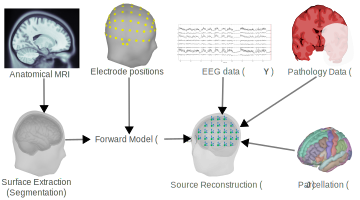
\includegraphics[width=0.8\textwidth]{figures/workflow}
%\caption{Formulation of inverse problem.}
\end{figure}
\end{block}

\begin{block}{Evaluation metrics}

Synthetic data protocol: one dipole is selected randomly, the known magnitude is set to {$\J_n(t)=\sin(2\pi t)$} at 15 Hz.

We tested 1,000 trials over different levels of noise against some classical methods: Tikhonov regularization and sLORETA \cite{survey2014}).

Parameters were selected via Generalized Cross-Validation \cite{siam_book}.
%
Brain cortex was parcellated using the Desikan-Killiani anatomical atlas.

\begin{wrapfigure}{r}{0.25\textwidth}
  \begin{center}
    \includegraphics[width=0.25\textwidth]{img/halfmax.png}
  \end{center}
\end{wrapfigure}

Performance was measured with tho following metrics:

%\begin{itemize}
%\item 
\textbf{Localization Error}. Source location is estimated as the center of mass of reconstructed $\J$,
$$
\text{pos}_{\text{source}} = \frac{\sum_{n=1}^N \nnorm{\hat{\J}_n} \text{pos}_n }{\sum_{n=1}^N \nnorm{\hat{\J}_n} }.
$$
%\item \textbf{Area Under Curve (AUC)}. Active sources are labeled as active/non-active using the normalized dipole magnitude and a parameter $\beta$
%$$
%\text{active}\ppar{\beta} = \sset{n; \frac{\nnorm{\J_n} \text{pos}_n }{\nnorm{\J_{MAX}} }<\beta }
%$$
%Labels obtained from simulated data are considered
%\item 
\textbf{Half-Max Size}. Measurement of dispersion,
$$
\text{HMS} = \text{vol}\sset{n; {\nnorm{\hat{\J}_n} } > \frac{1}{2}\nnorm{\hat{\J}_{MAX}}  }.
$$
%\end{itemize}

\begin{figure}
\centering
\includegraphics[width=0.4\textwidth]{img/boxplot_LocErr}
\includegraphics[width=0.4\textwidth]{img/boxplot_HMS}
%\caption{Formulation of inverse problem.}
\end{figure}

\end{block}

\end{column}

\separatorcolumn

\begin{column}{\colwidth}

\begin{block}{Results}

Missing due to a synchronization error with Google Drive.

\end{block}

\begin{block}{Future work}
We proposed a fast method to incorporate binary pathology data, obtained post-mortem, to enhance source localization based on EEG.

For this work we assumed that the damaged region is constant over time. 
However, this method can be easily extended to consider a time-changing damaged region.

Extensions of this method with other types of data as prior is being investigates.

\end{block}

  \begin{block}{References}
%    \nocite{*}
    \footnotesize{\bibliographystyle{abbrv}\bibliography{poster}}

  \end{block}

\end{column}

\separatorcolumn
\end{columns}
\end{frame}

\end{document}
